% GENERATED by scripts/make_pyramid_concept.py from pbl_assumptions_pyramid_split_vertical_colour.tex -- do not edit.
% =============================================================================
%  The assumptions of a one-dimensional PBL closure, as a pyramid -- VERTICAL, COLOUR-CODED version
%  GENERATED by scripts/make_pyramid_colour.py from pbl_assumptions_pyramid_split_vertical.tex (itself generated by make_pyramid_vertical.py from pbl_assumptions_pyramid_split.tex; edit the
%  horizontal file and regenerate. Tiers are columns (physics | concepts | formalism); a block
%  touches at its left exactly what it relies on. Scale: 0.86 cm per old cm along the ground,
%  column widths [2.5, 4.18, 5.3] cm for premises, concepts, formalism. Build: tectonic pbl_assumptions_pyramid_vertical.tex
% =============================================================================
\documentclass[10pt,border=1mm]{standalone}
\usepackage{iftex}
\ifPDFTeX
  \usepackage[utf8]{inputenc}
  \usepackage[T1]{fontenc}
  \usepackage{lmodern}
\else
  \usepackage{fontspec}
  \setmainfont{lmroman10-regular.otf}[BoldFont=lmroman10-bold.otf,
    ItalicFont=lmroman10-italic.otf, BoldItalicFont=lmroman10-bolditalic.otf]
\fi
\usepackage[british]{babel}
\usepackage{amsmath,amssymb}
\usepackage{xcolor}
\usepackage{tikz}
\usepackage{microtype}
\pagestyle{empty}
\setlength{\parindent}{0pt}
\setlength{\parskip}{0.5ex}
% rigid math relation spacing: the centred block texts would otherwise stretch around = and <<
\thickmuskip=5mu \medmuskip=4mu \thinmuskip=3mu

% ---- notation ---------------------------------------------------------------
\newcommand{\avg}[1]{\langle #1 \rangle}
\newcommand{\pd}[2]{\partial #1/\partial #2}
\newcommand{\qsq}{q^{2}}
\newcommand{\Rfc}{R_{fc}}
\newcommand{\dx}{\Delta x}
% ---- rows the PhD concept turns on (same data as the note's macros.tex) ------
\definecolor{cKey}{HTML}{7B2D8E}
\definecolor{cGXIX}{HTML}{990011}   % Goger 2019 port (the note's colour)
\definecolor{cFULL}{HTML}{7B2D8E}   % Kosovic-Juliano 3D closure (the note's colour)
% \hl{x0}{x1}{y0}{y1}{colour}{inset}: a frame inside a block, marking a scheme's decisive block
\newcommand{\hl}[6]{\draw[#5, line width=1.1pt] (#1+#6,#3+#6) rectangle (#2-#6,#4-#6);}
\newcommand{\setkey}[2]{\expandafter\def\csname key@#1\endcsname{#2}}
\makeatletter
\setkey{A1}{1}\setkey{B1}{1}\setkey{B2}{1}\setkey{B3}{1}\setkey{C3}{1}\setkey{C4}{1}\setkey{C6}{1}\setkey{C7}{1}
\setkey{B5}{2}\setkey{B6}{2}\setkey{C2}{2}\setkey{C5}{2}\setkey{C9}{2}
\newcommand{\keymark}[1]{\ifcsname key@#1\endcsname
  \if1\csname key@#1\endcsname\textcolor{cKey}{$\blacktriangleright$}\else\textcolor{cKey}{$\triangleright$}\fi\fi}
\makeatother
\newcommand{\pid}[1]{\keymark{#1}\textbf{#1}}
% \pb{x0}{x1}{y0}{y1}{style}{text}: a block from (x0,y0) to (x1,y1), text centred
\newcommand{\pbf}[7]{\pgfmathsetmacro{\pbw}{#2-#1-#7}%
  \draw[#5] (#1,#3) rectangle (#2,#4);
  \node[align=center, font=\tiny, inner sep=0pt, text width=\pbw cm] at ({(#1+#2)/2},{(#3+#4)/2}) {#6};}
% \pbunion{style}{tx}{ty}{tw}{text}{pieces x0/x1/y0/y1,...}{outline (x,y) -- ...}: one block of several rectangles
\newcommand{\pbunion}[7]{\foreach \ux/\uX/\uy/\uY in {#6} {\fill[black!22] (\ux,\uy) rectangle (\uX,\uY);}
  \draw[#1, fill=none] #7 -- cycle;
  \node[align=center, font=\tiny, inner sep=0pt, text width=#4 cm] at (#2,#3) {#5};}
\newcommand{\pb}[6]{\pgfmathsetmacro{\pbw}{#2-#1-0.20}%
  \draw[#5] (#1,#3) rectangle (#2,#4);
  \node[align=center, font=\tiny, inner sep=0pt, text width=\pbw cm] at ({(#1+#2)/2},{(#3+#4)/2}) {#6};}


% ---- the hectometre-scale column (used by the VERTICAL version only; read by scripts/make_pyramid_vertical.py)
% \hecto{<formal statement title>}{<what becomes of it at Delta = 500 m over the Inn Valley>}; no-op here.
% Sources: the mountain and grey-zone columns of the note's Table I.1 and the project's own runs.
\newcommand{\hecto}[2]{}
\hecto{Grid means are ensemble means}{By day, the largest eddies (of size $z_i$) are partly resolved, so the grid mean is no longer an ensemble mean. The shear of these eddies then enters both the resolved and the subgrid production. At night, all eddies are far smaller than $\dx$ again.}
\hecto{Column approximation}{Across the valley, the jet's horizontal shear is a sizeable fraction of its vertical shear.}
\hecto{Vertical divergence only}{Horizontal flux divergences are as large as the vertical one; valley budgets close only with horizontal transport and advection.}
\hecto{Wall value of $\qsq$}{At night, the turbulence near the ground hinges on the wall value; the $u_*$ of the sonics gives an observed one to test it.}
\hecto{Level-2.5 truncation}{Valid in stable and weakly unstable air, not in free convection. In fast transitions, the flow changes faster than the eddies adjust.}
\hecto{Stability functions}{No scheme we compare switches the turbulence off at a critical Richardson number. In stable air, all schemes but 3d-full take $S_M$ and $S_H$ from the vertical gradients alone.}
\hecto{Surface fluxes and first level}{The first model level is no longer in a constant-flux layer: the katabatic jet maximum lies below it, and over forest it lies in the roughness sublayer.}
\hecto{Master length scale}{In a valley, neither $z_i$ nor the wall distance is well defined, and the horizontal eddies are limited by the valley width: one length is not enough.}
\hecto{Constant set}{The constants were fitted to flat, dry boundary layers; whether they hold in valley flows is untested.}
\hecto{One length for $K$ and $\varepsilon$}{The dissipation does not depend on the grid, whereas the subgrid energy does. For this reason, the dissipation length has to shrink with $\dx$.}
\hecto{Pressure terms}{Taking them as small is a strong assumption in complex terrain, and only the residual of a measured TKE budget can test it.}
\hecto{K-form fluxes}{By day, plumes carry heat partly against the local gradient. Where slope and valley winds meet, the stress may leave the direction of the shear.}
\hecto{Buoyancy term}{On a slope, the surface heat flux has a horizontal component that a purely vertical buoyancy term misses.}

% ---- dependencies the contact rule cannot draw (post-audit list; used by scripts/make_pyramid_graph.py). No-op here.
\newcommand{\lean}[3][2]{}  % \lean[weight]{child}{parent}; weight 3 load-bearing, 2 real (default), 1 bookkeeping
% grouped by child; the order within a child is the importance of the parent (2026-09-21, Elias): the colour page
% draws the first three of weight >= 2 as corner marks, bottom left first, then counter-clockwise; the block's text names the same.
% Weights (Elias 2026-09-21): 3 load-bearing (thick border), 2 real, 1 bookkeeping (listed, not drawn).
\lean[2]{Boundary-layer approximation}{Boussinesq}
\lean[3]{Energy cascade}{Stationarity}
\lean[2]{Energy cascade}{Mixing}
\lean[2]{Local equilibrium}{Locality}
\lean[2]{Local equilibrium}{Horizontal homogeneity}
\lean[2]{Monin--Obukhov similarity}{Horizontal homogeneity}
\lean[2]{Monin--Obukhov similarity}{Constant-flux layer}
\lean[2]{Mixing length}{Horizontal homogeneity}
\lean[2]{Mixing length}{Mixing}
\lean[2]{Locality}{Mixing}
\lean[2]{Eddy viscosity}{Mixing length}
\lean[1]{Eddy viscosity}{Locality}
\lean[2]{Return to isotropy}{Horizontal homogeneity}
\lean[3]{Stability functions}{Local equilibrium}
\lean[3]{Stability functions}{Buoyancy production}
\lean[2]{Stability functions}{Boundary-layer approximation}
\lean[1]{Stability functions}{Level-2.5 truncation}
\lean[1]{Stability functions}{Universal constants}
\lean[2]{Level-2.5 truncation}{Weak anisotropy}
\lean[2]{Buoyancy production}{Return to isotropy}
\lean[1]{Universal constants}{Reynolds decomposition}
\lean[1]{Vertical divergence only}{Spectral gap}
\lean[1]{Wall value of $\qsq$}{Universal constants}
\lean[3]{Master length scale}{Buoyancy term}
\lean[3]{Buoyancy term}{K-form fluxes}
\lean[1]{Pressure terms}{Universal constants}
\lean[1]{Pressure terms}{Locality}
\lean[3]{One length for $K$ and $\varepsilon$}{Master length scale}
\lean[3]{K-form fluxes}{Master length scale}
\lean[3]{K-form fluxes}{Stability functions}
% ---- scheme quicklook (moons above the formalism tier; scripts/make_moons.py rewrites the strip)
% \moon{<block title>}{K|P|D x4} in the order MYNN as run, G19 port, 3D-APPROX, 3D-FULL; from Table I.0 of the note:
% a block is K if all its rows are kept, D if all are dropped, else P. No-op here (data only).
\newcommand{\moon}[2]{}
\moon{Grid means are ensemble means}{P K P P}
\moon{Column approximation}{K P K D}
\moon{Vertical divergence only}{P P P D}   % MYNN P since 2026-10-26: the control advects TKE (Table 1 of the concept)
\moon{Wall value of $\qsq$}{K K D D}
\moon{Level-2.5 truncation}{K K K K}
\moon{Stability functions}{K P K D}   % 2026-10-26 (Elias): level-2.5 block, no cutoff in any scheme; G19 half (its HSP source knows no Ri), 3D-FULL has no S_M, S_H
\moon{Surface fluxes and first level}{K K K K}
\moon{Master length scale}{K P K K}
\moon{Constant set}{K K K K}
\moon{One length for $K$ and $\varepsilon$}{K K K K}
\moon{Pressure terms}{K K K K}
\moon{K-form fluxes}{K P P D}   % MYNN K since 2026-10-26: the control runs without mass flux (bl_mynn_edmf = 0)
\moon{Buoyancy term}{P P P P}
% glyphs (the note's), absolute size, colour = scheme identity
\newcommand{\gK}{\tikz[baseline=-0.6ex]{\fill (0,0) circle (0.11);}}
\newcommand{\gP}{\tikz[baseline=-0.6ex]{\draw[line width=0.5pt] (0,0) circle (0.11); \fill (0,0) -- (90:0.11) arc (90:270:0.11) -- cycle;}}
\newcommand{\gD}{\tikz[baseline=-0.6ex]{\draw[line width=0.5pt] (0,0) circle (0.11);}}
\definecolor{cMYNN}{HTML}{3A6B00}    % MYNN as run
\definecolor{cAPPROX}{HTML}{9A5AA8}  % 3D-APPROX


% vertical block: rectangle + centred text, text width = block width - hpad
\newcommand{\pbv}[7]{\pgfmathsetmacro{\pbw}{#2-#1-#7}%
  \draw[#5] (#1,#3) rectangle (#2,#4);
  \node[align=center, font=\fontsize{7}{7.5}\selectfont, inner sep=0pt, text width=\pbw cm] at ({(#1+#2)/2},{(#3+#4)/2}) {#6};}
\newcommand{\hlv}[6]{\draw[#5, line width=1.1pt] (#1+#6,#3+#6) rectangle (#2-#6,#4-#6);}
% compound blocks in the page's text size
\renewcommand{\pbunion}[7]{\foreach \ux/\uX/\uy/\uY in {#6} {\fill[#1] (\ux,\uy) rectangle (\uX,\uY);}
  \draw[bk] #7 -- cycle;
  \node[align=center, font=\fontsize{7}{7.5}\selectfont, inner sep=0pt, text width=#4 cm] at (#2,#3) {#5};}
% hectometre box: dashed, left-aligned commentary beside a concept (not a block of the chain)
\newcommand{\pbh}[5]{\pgfmathsetmacro{\pbw}{#2-#1-0.30}%
  \draw[hecto] (#1,#3) rectangle (#2,#4);
  \node[align=left, font=\fontsize{6.5}{7.6}\selectfont, inner sep=0pt, text width=\pbw cm] at ({(#1+#2)/2},{(#3+#4)/2}) {#5};}

% ---- block colours (OKLCH: hue by vertical position, lightness by column) ----
\definecolor{blk0}{rgb}{0.8545,0.5175,0.4467} % Spectral gap
\definecolor{blk1}{rgb}{0.8376,0.5372,0.3721} % Mixing
\definecolor{blk2}{rgb}{0.4972,0.6827,0.4078} % Stationarity
\definecolor{blk3}{rgb}{0.2395,0.7082,0.6233} % Similarity
\definecolor{blk4}{rgb}{0.7368,0.6027,0.2739} % Horizontal homogeneity
\definecolor{blk5}{rgb}{0.2402,0.6799,0.8125} % Small-scale isotropy
\definecolor{blk6}{rgb}{0.4113,0.6377,0.8811} % Weak anisotropy
\definecolor{blk7}{rgb}{0.5139,0.6074,0.8911} % Gradient scale
\definecolor{blk8}{rgb}{0.6180,0.5734,0.8709} % Axisymmetric mixing
\definecolor{blk9}{rgb}{0.7075,0.5427,0.8189} % Boussinesq
\definecolor{blk10}{rgb}{0.9958,0.6757,0.6067} % Reynolds decomposition
\definecolor{blk11}{rgb}{0.9853,0.6948,0.4904} % Ergodicity in space
\definecolor{blk12}{rgb}{0.8762,0.7579,0.4257} % Boundary-layer approximation
\definecolor{blk13}{rgb}{0.7500,0.8060,0.4741} % Constant-flux layer
\definecolor{blk14}{rgb}{0.6512,0.8322,0.5444} % Local equilibrium
\definecolor{blk15}{rgb}{0.5014,0.8562,0.6747} % Monin--Obukhov similarity
\definecolor{blk16}{rgb}{0.4003,0.8607,0.7884} % Mixing length
\definecolor{blk17}{rgb}{0.3656,0.8526,0.8837} % Universal constants
\definecolor{blk18}{rgb}{0.4078,0.8330,0.9660} % Energy cascade
\definecolor{blk19}{rgb}{0.5563,0.7977,0.9942} % Return to isotropy
\definecolor{blk20}{rgb}{0.7291,0.7435,0.9947} % Eddy viscosity
\definecolor{blk21}{rgb}{0.6693,0.7660,0.9890} % Locality
\definecolor{blk22}{rgb}{0.8310,0.6990,0.9964} % Buoyancy production
\definecolor{blk23}{rgb}{0.9898,0.8852,0.8304} % Grid means are ensemble means
\definecolor{blk24}{rgb}{0.9977,0.8931,0.7353} % Column approximation
\definecolor{blk25}{rgb}{0.9872,0.9133,0.5693} % Vertical divergence only
\definecolor{blk26}{rgb}{0.8737,0.9532,0.6207} % Wall value of $\qsq$
\definecolor{blk27}{rgb}{0.7719,0.9792,0.6942} % Level-2.5 truncation
\definecolor{blk28}{rgb}{0.6523,0.9992,0.8024} % Surface fluxes and first level
\definecolor{blk29}{rgb}{0.5971,0.9972,0.9210} % Master length scale
\definecolor{blk30}{rgb}{0.6526,0.9749,0.9947} % Constant set
\definecolor{blk31}{rgb}{0.7651,0.9451,0.9940} % One length for $K$ and $\varepsilon$
\definecolor{blk32}{rgb}{0.8252,0.9266,0.9898} % Pressure terms
\definecolor{blk33}{rgb}{0.8533,0.9172,0.9876} % Stability functions
\definecolor{blk34}{rgb}{0.8855,0.9049,0.9904} % K-form fluxes
\definecolor{blk35}{rgb}{0.9322,0.8853,0.9965} % Buoyancy term
\begin{document}
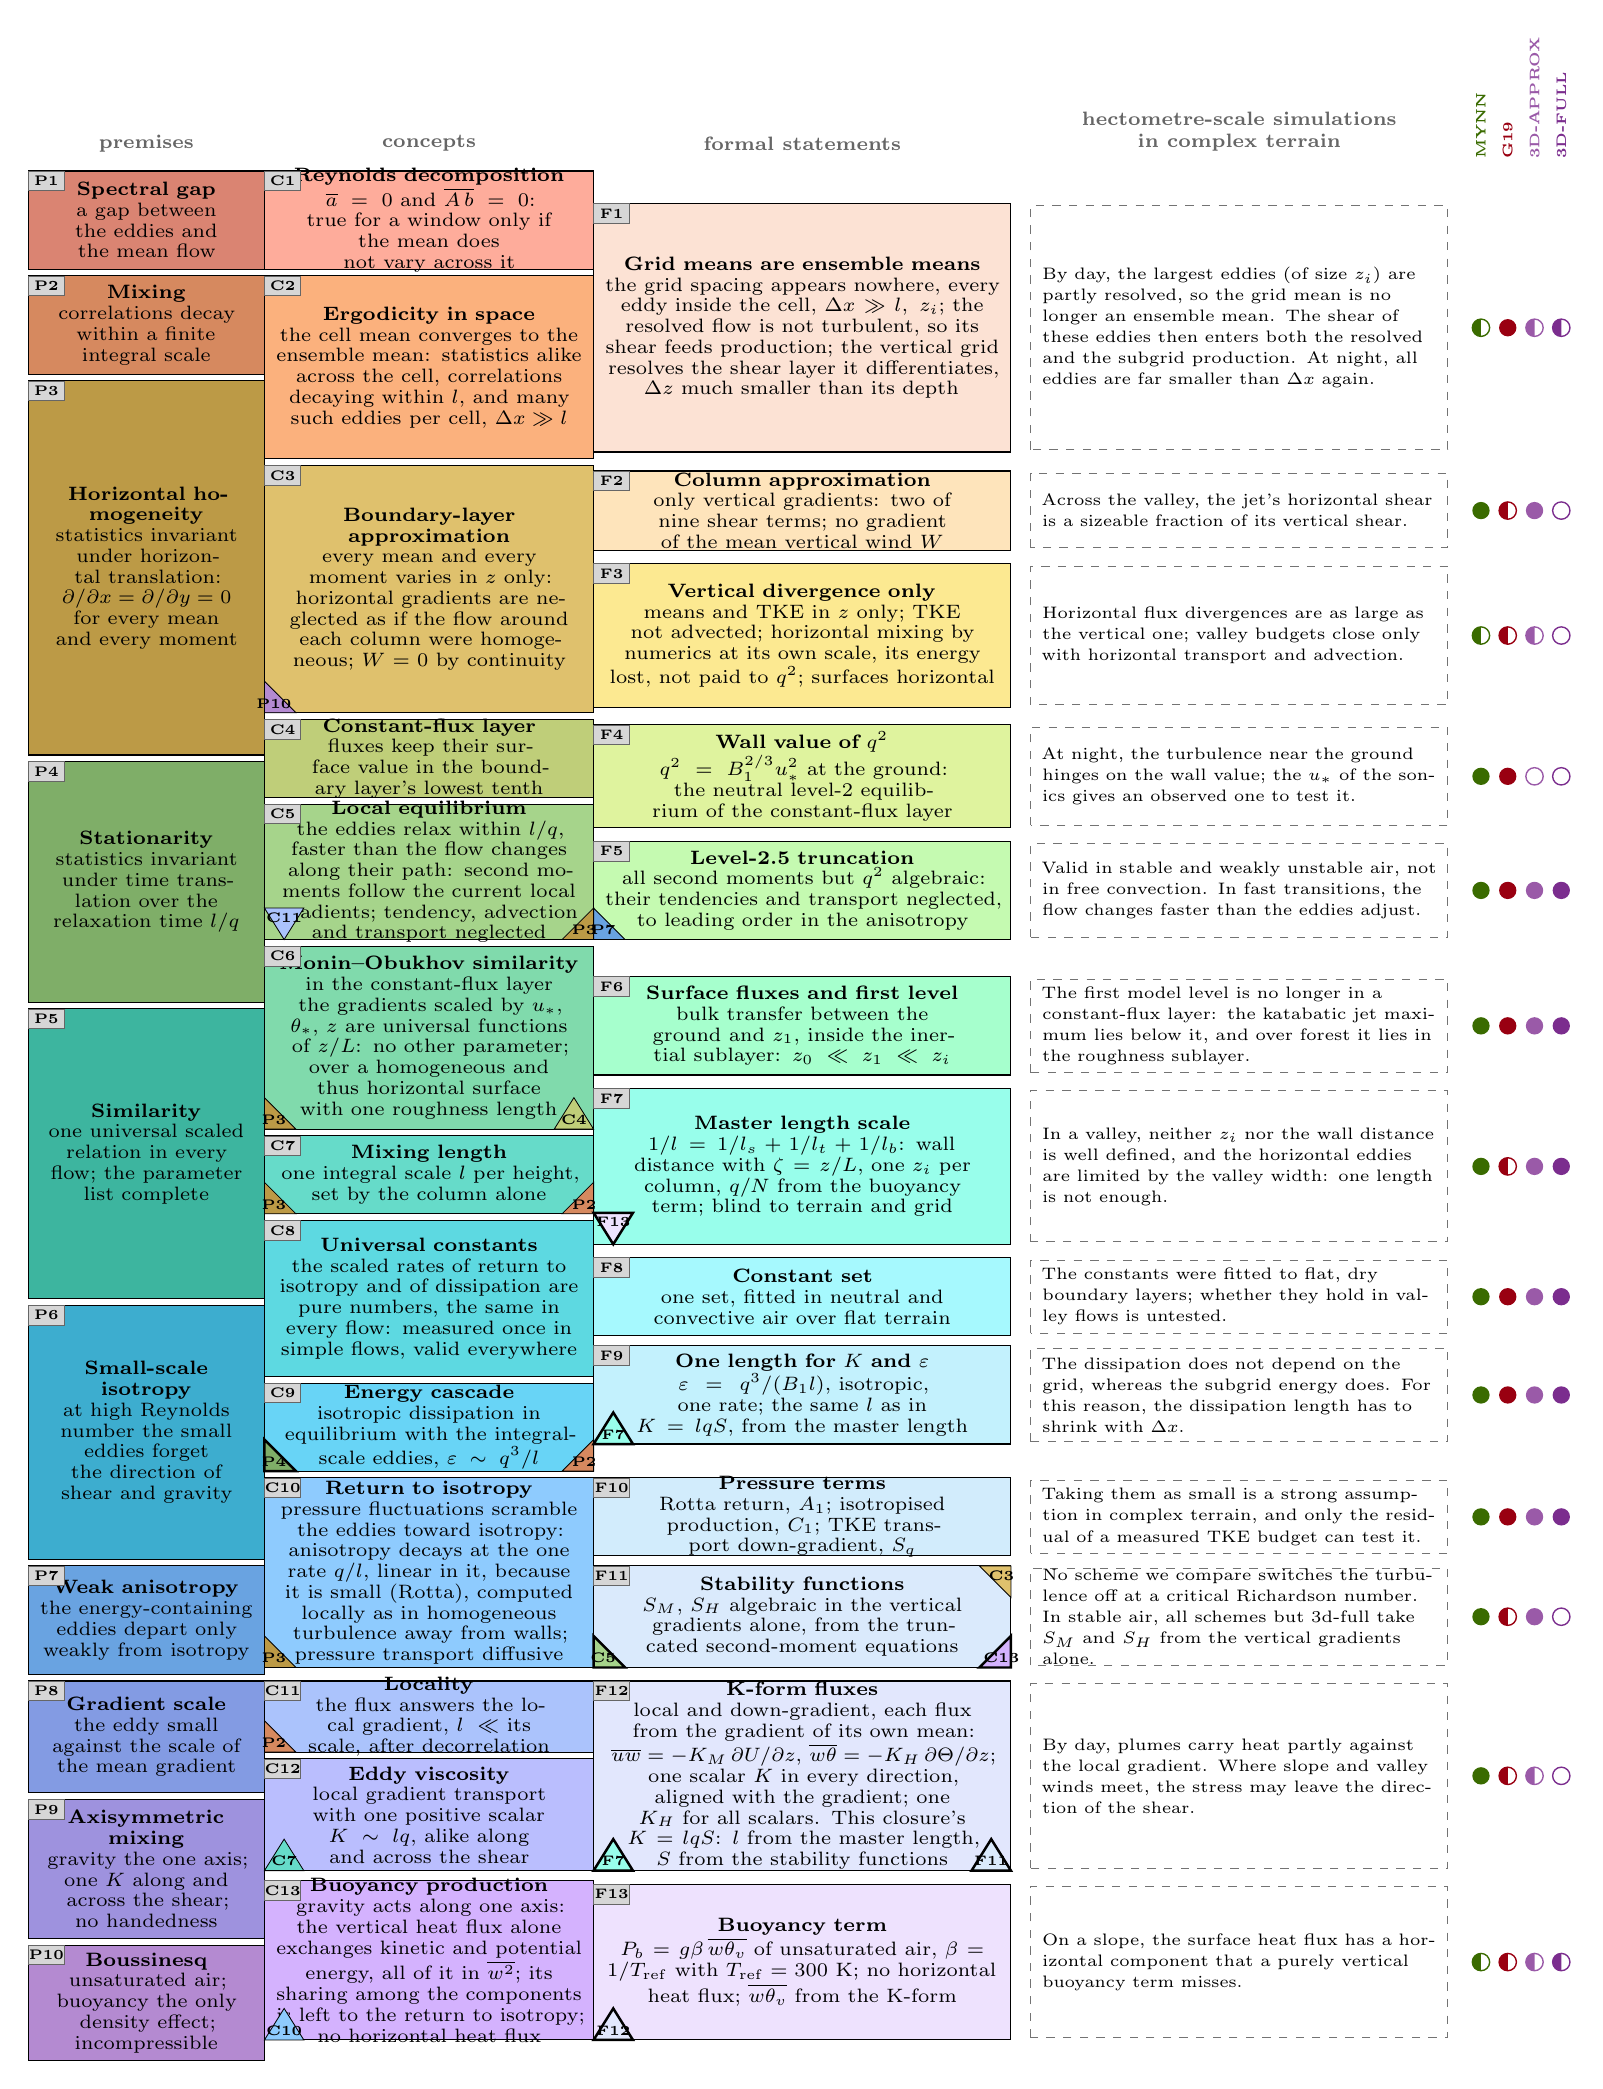
\begin{tikzpicture}[x=1cm, y=1cm,
  ground/.style={draw, line width=0.4pt, fill=black!22},
  hyp/.style={draw, line width=0.4pt, fill=black!9},
  row/.style={draw, line width=0.4pt, fill=white},
  bk/.style={draw, line width=0.4pt},
  hecto/.style={draw=black!55, dashed, line width=0.4pt, fill=white}]
\node[font=\scriptsize\bfseries, text=black!60] at (1.500,23.871) {premises};
\node[font=\scriptsize\bfseries, text=black!60] at (5.090,23.871) {concepts};
\node[font=\scriptsize\bfseries, text=black!60] at (9.830,23.871) {formal statements};
\node[font=\fontsize{5}{5.5}\selectfont\bfseries, text=cMYNN, rotate=90, anchor=west] at (18.450,23.55) {MYNN};
\node[font=\fontsize{5}{5.5}\selectfont\bfseries, text=cGXIX, rotate=90, anchor=west] at (18.790,23.55) {G19};
\node[font=\fontsize{5}{5.5}\selectfont\bfseries, text=cAPPROX, rotate=90, anchor=west] at (19.130,23.55) {3D-APPROX};
\node[font=\fontsize{5}{5.5}\selectfont\bfseries, text=cFULL, rotate=90, anchor=west] at (19.470,23.55) {3D-FULL};
\node[font=\scriptsize\bfseries, text=black!60, align=center] at (15.380,24.021) {hectometre-scale simulations\\ in complex terrain};
\pbv{0.000}{3.000}{22.274}{23.521}{bk, fill=blk0}{\textbf{Spectral gap}\\ a gap between the eddies and the mean flow}{0.30}
\pbv{0.000}{3.000}{20.941}{22.188}{bk, fill=blk1}{\textbf{Mixing}\\ correlations decay within a finite integral scale}{0.30}
\pbv{0.000}{3.000}{12.965}{16.018}{bk, fill=blk2}{\textbf{Stationarity}\\ statistics invariant under time translation over the relaxation time $l/q$}{0.30}
\pbv{0.000}{3.000}{9.202}{12.879}{bk, fill=blk3}{\textbf{Similarity}\\ one universal scaled relation in every flow; the parameter list complete}{0.30}
\pbv{0.000}{3.000}{16.104}{20.855}{bk, fill=blk4}{\textbf{Horizontal homogeneity}\\ statistics invariant under horizontal translation: \mbox{$\partial/\partial x = \partial/\partial y = 0$} for every mean and every moment}{0.30}
\pbv{0.000}{3.000}{5.891}{9.116}{bk, fill=blk5}{\textbf{Small-scale isotropy}\\ at high Reynolds number the small eddies forget the direction of shear and gravity}{0.30}
\pbv{0.000}{3.000}{4.429}{5.805}{bk, fill=blk6}{\textbf{Weak anisotropy}\\ the energy-containing eddies depart only weakly from isotropy}{0.30}
\pbv{0.000}{3.000}{2.924}{4.343}{bk, fill=blk7}{\textbf{Gradient scale}\\ the eddy small against the scale of the mean gradient}{0.30}
\pbv{0.000}{3.000}{1.075}{2.838}{bk, fill=blk8}{\textbf{Axisymmetric mixing}\\ gravity the one axis; one $K$ along and across the shear; no handedness}{0.30}
\pbv{0.000}{3.000}{-0.473}{0.989}{bk, fill=blk9}{\textbf{Boussinesq}\\ unsaturated air; buoyancy the only density effect; incompressible}{0.30}
\pbv{3.000}{7.180}{22.274}{23.521}{bk, fill=blk10}{\textbf{Reynolds decomposition}\\ $\overline{a} = 0$ and $\overline{A\,b} = 0$:\\ true for a window only if\\ the mean does not vary across it}{0.30}
\pbv{3.000}{7.180}{19.866}{22.188}{bk, fill=blk11}{\textbf{Ergodicity in space}\\ the cell mean converges to the ensemble mean: statistics alike across the cell, correlations decaying within $l$, and many such eddies per cell, \mbox{$\dx \gg l$}}{0.30}
\pbv{3.000}{7.180}{16.641}{19.780}{bk, fill=blk12}{\textbf{Boundary-layer approximation}\\ every mean and every moment varies in $z$ only: horizontal gradients are neglected as if the flow around each column were homogeneous; $W = 0$ by continuity}{0.56}
\pbv{3.000}{7.180}{15.566}{16.555}{bk, fill=blk13}{\textbf{Constant-flux layer}\\ fluxes keep their surface value in the boundary layer's lowest tenth}{0.30}
\pbv{3.000}{7.180}{13.760}{15.480}{bk, fill=blk14}{\textbf{Local equilibrium}\\ the eddies relax within $l/q$, faster than the flow changes along their path: second moments follow the current local gradients; tendency, advection and transport neglected}{0.30}
\pbv{3.000}{7.180}{11.352}{13.674}{bk, fill=blk15}{\textbf{Monin--Obukhov similarity}\\ in the constant-flux layer the gradients scaled by $u_*$, $\theta_*$, $z$ are universal functions of $z/L$: no other parameter; over a homogeneous and thus horizontal surface with one roughness length}{0.30}
\pbv{3.000}{7.180}{10.277}{11.266}{bk, fill=blk16}{\textbf{Mixing length}\\ one integral scale $l$ per height, set by the column alone}{0.30}
\pbv{3.000}{7.180}{8.213}{10.191}{bk, fill=blk17}{\textbf{Universal constants}\\ the scaled rates of return to isotropy and of dissipation are pure numbers, the same in every flow: measured once in simple flows, valid everywhere}{0.30}
\pbv{3.000}{7.180}{7.009}{8.127}{bk, fill=blk18}{\textbf{Energy cascade}\\ isotropic dissipation in equilibrium with the integral-scale eddies, $\varepsilon \sim q^3/l$}{0.30}
\pbv{3.000}{7.180}{4.515}{6.923}{bk, fill=blk19}{\textbf{Return to isotropy}\\ pressure fluctuations scramble the eddies toward isotropy: anisotropy decays at the one rate $q/l$, linear in it, because it is small (Rotta), computed locally as in homogeneous turbulence away from walls; pressure transport diffusive}{0.30}
\pbv{3.000}{7.180}{1.935}{3.354}{bk, fill=blk20}{\textbf{Eddy viscosity}\\ local gradient transport with one positive scalar $K \sim l q$, alike along and across the shear}{0.40}
\pbv{3.000}{7.180}{3.440}{4.343}{bk, fill=blk21}{\textbf{Locality}\\ the flux answers the local gradient, $l \ll$ its scale, after decorrelation}{0.30}
\pbv{3.000}{7.180}{-0.215}{1.806}{bk, fill=blk22}{\textbf{Buoyancy production}\\ gravity acts along one axis: the vertical heat flux alone exchanges kinetic and potential energy, all of it in $\overline{w^2}$; its sharing among the components is left to the return to isotropy; no horizontal heat flux}{0.30}
\pbv{7.180}{12.480}{19.952}{23.108}{bk, fill=blk23}{\textbf{Grid means are ensemble means}\\ the grid spacing appears nowhere, every eddy inside the cell, $\dx \gg l,\ z_i$; the resolved flow is not turbulent, so its shear feeds production; the vertical grid resolves the shear layer it differentiates, $\Delta z$ much smaller than its depth}{0.30}
\pbv{7.180}{12.480}{18.705}{19.711}{bk, fill=blk24}{\textbf{Column approximation}\\ only vertical gradients: two of nine shear terms; no gradient of the mean vertical wind $W$}{0.56}
\pbv{7.180}{12.480}{16.710}{18.533}{bk, fill=blk25}{\textbf{Vertical divergence only}\\ means and TKE in $z$ only; TKE not advected; horizontal mixing by numerics at its own scale, its energy lost, not paid to $\qsq$; surfaces horizontal}{0.40}
\pbv{7.180}{12.480}{15.179}{16.486}{bk, fill=blk26}{\textbf{Wall value of $\qsq$}\\ $\qsq = B_1^{2/3} u_*^2$ at the ground: the neutral level-2 equilibrium of the constant-flux layer}{0.30}
\pbv{7.180}{12.480}{13.760}{15.007}{bk, fill=blk27}{\textbf{Level-2.5 truncation}\\ all second moments but $\qsq$ algebraic: their tendencies and transport neglected, to leading order in the anisotropy}{0.30}
\pbv{7.180}{12.480}{12.040}{13.287}{bk, fill=blk28}{\textbf{Surface fluxes and first level}\\ bulk transfer between the ground and $z_1$, inside the inertial sublayer: $z_0 \ll z_1 \ll z_i$}{0.30}
\pbv{7.180}{12.480}{9.890}{11.868}{bk, fill=blk29}{\textbf{Master length scale}\\ $1/l = 1/l_s + 1/l_t + 1/l_b$: wall distance with $\zeta = z/L$, one $z_i$ per column, $q/N$ from the buoyancy term; blind to terrain and grid}{0.56}
\pbv{7.180}{12.480}{8.729}{9.718}{bk, fill=blk30}{\textbf{Constant set}\\ one set, fitted in neutral and convective air over flat terrain}{0.30}
\pbv{7.180}{12.480}{7.353}{8.600}{bk, fill=blk31}{\textbf{One length for $K$ and $\varepsilon$}\\ $\varepsilon = q^3/(B_1 l)$, isotropic, one rate; the same $l$ as in $K = lqS$, from the master length}{0.30}
\pbv{7.180}{12.480}{5.934}{6.923}{bk, fill=blk32}{\textbf{Pressure terms}\\ Rotta return, $A_1$; isotropised production, $C_1$; TKE transport down-gradient, $S_q$}{0.30}
\pbv{7.180}{12.480}{4.515}{5.805}{bk, fill=blk33}{\textbf{Stability functions}\\ $S_M$, $S_H$ algebraic in the vertical gradients alone, from the truncated second-moment equations}{0.56}
\pbv{7.180}{12.480}{1.935}{4.343}{bk, fill=blk34}{\textbf{K-form fluxes}\\ local and down-gradient, each flux from the gradient of its own mean: \mbox{$\overline{uw} = -K_M\,\partial U/\partial z$}, \mbox{$\overline{w\theta} = -K_H\,\partial\Theta/\partial z$}; one scalar $K$ in every direction, aligned with the gradient; one $K_H$ for all scalars. This closure's $K = lqS$: $l$ from the master length, $S$ from the stability functions}{0.40}
\pbv{7.180}{12.480}{-0.215}{1.763}{bk, fill=blk35}{\textbf{Buoyancy term}\\ $P_b = g\beta\,\overline{w\theta_v}$ of unsaturated air, $\beta = 1/T_\mathrm{ref}$ with $T_\mathrm{ref} = 300$~K; no horizontal heat flux; $\overline{w\theta_v}$ from the K-form}{0.30}
\node[inner sep=0pt] at (18.450,21.530) {\color{cMYNN}\gP};
\node[inner sep=0pt] at (18.790,21.530) {\color{cGXIX}\gK};
\node[inner sep=0pt] at (19.130,21.530) {\color{cAPPROX}\gP};
\node[inner sep=0pt] at (19.470,21.530) {\color{cFULL}\gP};
\node[inner sep=0pt] at (18.450,19.208) {\color{cMYNN}\gK};
\node[inner sep=0pt] at (18.790,19.208) {\color{cGXIX}\gP};
\node[inner sep=0pt] at (19.130,19.208) {\color{cAPPROX}\gK};
\node[inner sep=0pt] at (19.470,19.208) {\color{cFULL}\gD};
\node[inner sep=0pt] at (18.450,17.621) {\color{cMYNN}\gP};
\node[inner sep=0pt] at (18.790,17.621) {\color{cGXIX}\gP};
\node[inner sep=0pt] at (19.130,17.621) {\color{cAPPROX}\gP};
\node[inner sep=0pt] at (19.470,17.621) {\color{cFULL}\gD};
\node[inner sep=0pt] at (18.450,15.833) {\color{cMYNN}\gK};
\node[inner sep=0pt] at (18.790,15.833) {\color{cGXIX}\gK};
\node[inner sep=0pt] at (19.130,15.833) {\color{cAPPROX}\gD};
\node[inner sep=0pt] at (19.470,15.833) {\color{cFULL}\gD};
\node[inner sep=0pt] at (18.450,14.384) {\color{cMYNN}\gK};
\node[inner sep=0pt] at (18.790,14.384) {\color{cGXIX}\gK};
\node[inner sep=0pt] at (19.130,14.384) {\color{cAPPROX}\gK};
\node[inner sep=0pt] at (19.470,14.384) {\color{cFULL}\gK};
\node[inner sep=0pt] at (18.450,12.664) {\color{cMYNN}\gK};
\node[inner sep=0pt] at (18.790,12.664) {\color{cGXIX}\gK};
\node[inner sep=0pt] at (19.130,12.664) {\color{cAPPROX}\gK};
\node[inner sep=0pt] at (19.470,12.664) {\color{cFULL}\gK};
\node[inner sep=0pt] at (18.450,10.879) {\color{cMYNN}\gK};
\node[inner sep=0pt] at (18.790,10.879) {\color{cGXIX}\gP};
\node[inner sep=0pt] at (19.130,10.879) {\color{cAPPROX}\gK};
\node[inner sep=0pt] at (19.470,10.879) {\color{cFULL}\gK};
\node[inner sep=0pt] at (18.450,9.224) {\color{cMYNN}\gK};
\node[inner sep=0pt] at (18.790,9.224) {\color{cGXIX}\gK};
\node[inner sep=0pt] at (19.130,9.224) {\color{cAPPROX}\gK};
\node[inner sep=0pt] at (19.470,9.224) {\color{cFULL}\gK};
\node[inner sep=0pt] at (18.450,7.976) {\color{cMYNN}\gK};
\node[inner sep=0pt] at (18.790,7.976) {\color{cGXIX}\gK};
\node[inner sep=0pt] at (19.130,7.976) {\color{cAPPROX}\gK};
\node[inner sep=0pt] at (19.470,7.976) {\color{cFULL}\gK};
\node[inner sep=0pt] at (18.450,6.428) {\color{cMYNN}\gK};
\node[inner sep=0pt] at (18.790,6.428) {\color{cGXIX}\gK};
\node[inner sep=0pt] at (19.130,6.428) {\color{cAPPROX}\gK};
\node[inner sep=0pt] at (19.470,6.428) {\color{cFULL}\gK};
\node[inner sep=0pt] at (18.450,5.160) {\color{cMYNN}\gK};
\node[inner sep=0pt] at (18.790,5.160) {\color{cGXIX}\gP};
\node[inner sep=0pt] at (19.130,5.160) {\color{cAPPROX}\gK};
\node[inner sep=0pt] at (19.470,5.160) {\color{cFULL}\gD};
\node[inner sep=0pt] at (18.450,3.139) {\color{cMYNN}\gK};
\node[inner sep=0pt] at (18.790,3.139) {\color{cGXIX}\gP};
\node[inner sep=0pt] at (19.130,3.139) {\color{cAPPROX}\gP};
\node[inner sep=0pt] at (19.470,3.139) {\color{cFULL}\gD};
\node[inner sep=0pt] at (18.450,0.774) {\color{cMYNN}\gP};
\node[inner sep=0pt] at (18.790,0.774) {\color{cGXIX}\gP};
\node[inner sep=0pt] at (19.130,0.774) {\color{cAPPROX}\gP};
\node[inner sep=0pt] at (19.470,0.774) {\color{cFULL}\gP};
\pbh{12.730}{18.030}{19.982}{23.078}{By day, the largest eddies (of size $z_i$) are partly resolved, so the grid mean is no longer an ensemble mean. The shear of these eddies then enters both the resolved and the subgrid production. At night, all eddies are far smaller than $\dx$ again.}
\pbh{12.730}{18.030}{18.735}{19.681}{Across the valley, the jet's horizontal shear is a sizeable fraction of its vertical shear.}
\pbh{12.730}{18.030}{16.740}{18.503}{Horizontal flux divergences are as large as the vertical one; valley budgets close only with horizontal transport and advection.}
\pbh{12.730}{18.030}{15.209}{16.456}{At night, the turbulence near the ground hinges on the wall value; the $u_*$ of the sonics gives an observed one to test it.}
\pbh{12.730}{18.030}{13.790}{14.977}{Valid in stable and weakly unstable air, not in free convection. In fast transitions, the flow changes faster than the eddies adjust.}
\pbh{12.730}{18.030}{12.070}{13.257}{The first model level is no longer in a constant-flux layer: the katabatic jet maximum lies below it, and over forest it lies in the roughness sublayer.}
\pbh{12.730}{18.030}{9.920}{11.838}{In a valley, neither $z_i$ nor the wall distance is well defined, and the horizontal eddies are limited by the valley width: one length is not enough.}
\pbh{12.730}{18.030}{8.759}{9.688}{The constants were fitted to flat, dry boundary layers; whether they hold in valley flows is untested.}
\pbh{12.730}{18.030}{7.383}{8.570}{The dissipation does not depend on the grid, whereas the subgrid energy does. For this reason, the dissipation length has to shrink with $\dx$.}
\pbh{12.730}{18.030}{5.964}{6.893}{Taking them as small is a strong assumption in complex terrain, and only the residual of a measured TKE budget can test it.}
\pbh{12.730}{18.030}{4.545}{5.775}{No scheme we compare switches the turbulence off at a critical Richardson number. In stable air, all schemes but 3d-full take $S_M$ and $S_H$ from the vertical gradients alone.}
\pbh{12.730}{18.030}{1.965}{4.313}{By day, plumes carry heat partly against the local gradient. Where slope and valley winds meet, the stress may leave the direction of the shear.}
\pbh{12.730}{18.030}{-0.185}{1.733}{On a slope, the surface heat flux has a horizontal component that a purely vertical buoyancy term misses.}
% ---- shortcut tabs ----
\fill[black!16] (0.000,23.271) rectangle (0.460,23.521); \draw[black!60, line width=0.25pt] (0.000,23.271) rectangle (0.460,23.521); \node[inner sep=0pt, font=\fontsize{5.5}{6}\selectfont\bfseries] at (0.230,23.396) {P1}; % Spectral gap
\fill[black!16] (0.000,21.938) rectangle (0.460,22.188); \draw[black!60, line width=0.25pt] (0.000,21.938) rectangle (0.460,22.188); \node[inner sep=0pt, font=\fontsize{5.5}{6}\selectfont\bfseries] at (0.230,22.063) {P2}; % Mixing
\fill[black!16] (0.000,15.768) rectangle (0.460,16.018); \draw[black!60, line width=0.25pt] (0.000,15.768) rectangle (0.460,16.018); \node[inner sep=0pt, font=\fontsize{5.5}{6}\selectfont\bfseries] at (0.230,15.893) {P4}; % Stationarity
\fill[black!16] (0.000,12.629) rectangle (0.460,12.879); \draw[black!60, line width=0.25pt] (0.000,12.629) rectangle (0.460,12.879); \node[inner sep=0pt, font=\fontsize{5.5}{6}\selectfont\bfseries] at (0.230,12.754) {P5}; % Similarity
\fill[black!16] (0.000,20.605) rectangle (0.460,20.855); \draw[black!60, line width=0.25pt] (0.000,20.605) rectangle (0.460,20.855); \node[inner sep=0pt, font=\fontsize{5.5}{6}\selectfont\bfseries] at (0.230,20.730) {P3}; % Horizontal homogeneity
\fill[black!16] (0.000,8.866) rectangle (0.460,9.116); \draw[black!60, line width=0.25pt] (0.000,8.866) rectangle (0.460,9.116); \node[inner sep=0pt, font=\fontsize{5.5}{6}\selectfont\bfseries] at (0.230,8.991) {P6}; % Small-scale isotropy
\fill[black!16] (0.000,5.555) rectangle (0.460,5.805); \draw[black!60, line width=0.25pt] (0.000,5.555) rectangle (0.460,5.805); \node[inner sep=0pt, font=\fontsize{5.5}{6}\selectfont\bfseries] at (0.230,5.680) {P7}; % Weak anisotropy
\fill[black!16] (0.000,4.093) rectangle (0.460,4.343); \draw[black!60, line width=0.25pt] (0.000,4.093) rectangle (0.460,4.343); \node[inner sep=0pt, font=\fontsize{5.5}{6}\selectfont\bfseries] at (0.230,4.218) {P8}; % Gradient scale
\fill[black!16] (0.000,2.588) rectangle (0.460,2.838); \draw[black!60, line width=0.25pt] (0.000,2.588) rectangle (0.460,2.838); \node[inner sep=0pt, font=\fontsize{5.5}{6}\selectfont\bfseries] at (0.230,2.713) {P9}; % Axisymmetric mixing
\fill[black!16] (0.000,0.739) rectangle (0.460,0.989); \draw[black!60, line width=0.25pt] (0.000,0.739) rectangle (0.460,0.989); \node[inner sep=0pt, font=\fontsize{5.5}{6}\selectfont\bfseries] at (0.230,0.864) {P10}; % Boussinesq
\fill[black!16] (3.000,23.271) rectangle (3.460,23.521); \draw[black!60, line width=0.25pt] (3.000,23.271) rectangle (3.460,23.521); \node[inner sep=0pt, font=\fontsize{5.5}{6}\selectfont\bfseries] at (3.230,23.396) {C1}; % Reynolds decomposition
\fill[black!16] (3.000,21.938) rectangle (3.460,22.188); \draw[black!60, line width=0.25pt] (3.000,21.938) rectangle (3.460,22.188); \node[inner sep=0pt, font=\fontsize{5.5}{6}\selectfont\bfseries] at (3.230,22.063) {C2}; % Ergodicity in space
\fill[black!16] (3.000,19.530) rectangle (3.460,19.780); \draw[black!60, line width=0.25pt] (3.000,19.530) rectangle (3.460,19.780); \node[inner sep=0pt, font=\fontsize{5.5}{6}\selectfont\bfseries] at (3.230,19.655) {C3}; % Boundary-layer approximation
\fill[black!16] (3.000,16.305) rectangle (3.460,16.555); \draw[black!60, line width=0.25pt] (3.000,16.305) rectangle (3.460,16.555); \node[inner sep=0pt, font=\fontsize{5.5}{6}\selectfont\bfseries] at (3.230,16.430) {C4}; % Constant-flux layer
\fill[black!16] (3.000,15.230) rectangle (3.460,15.480); \draw[black!60, line width=0.25pt] (3.000,15.230) rectangle (3.460,15.480); \node[inner sep=0pt, font=\fontsize{5.5}{6}\selectfont\bfseries] at (3.230,15.355) {C5}; % Local equilibrium
\fill[black!16] (3.000,13.424) rectangle (3.460,13.674); \draw[black!60, line width=0.25pt] (3.000,13.424) rectangle (3.460,13.674); \node[inner sep=0pt, font=\fontsize{5.5}{6}\selectfont\bfseries] at (3.230,13.549) {C6}; % Monin--Obukhov similarity
\fill[black!16] (3.000,11.016) rectangle (3.460,11.266); \draw[black!60, line width=0.25pt] (3.000,11.016) rectangle (3.460,11.266); \node[inner sep=0pt, font=\fontsize{5.5}{6}\selectfont\bfseries] at (3.230,11.141) {C7}; % Mixing length
\fill[black!16] (3.000,9.941) rectangle (3.460,10.191); \draw[black!60, line width=0.25pt] (3.000,9.941) rectangle (3.460,10.191); \node[inner sep=0pt, font=\fontsize{5.5}{6}\selectfont\bfseries] at (3.230,10.066) {C8}; % Universal constants
\fill[black!16] (3.000,7.877) rectangle (3.460,8.127); \draw[black!60, line width=0.25pt] (3.000,7.877) rectangle (3.460,8.127); \node[inner sep=0pt, font=\fontsize{5.5}{6}\selectfont\bfseries] at (3.230,8.002) {C9}; % Energy cascade
\fill[black!16] (3.000,6.673) rectangle (3.460,6.923); \draw[black!60, line width=0.25pt] (3.000,6.673) rectangle (3.460,6.923); \node[inner sep=0pt, font=\fontsize{5.5}{6}\selectfont\bfseries] at (3.230,6.798) {C10}; % Return to isotropy
\fill[black!16] (3.000,3.104) rectangle (3.460,3.354); \draw[black!60, line width=0.25pt] (3.000,3.104) rectangle (3.460,3.354); \node[inner sep=0pt, font=\fontsize{5.5}{6}\selectfont\bfseries] at (3.230,3.229) {C12}; % Eddy viscosity
\fill[black!16] (3.000,4.093) rectangle (3.460,4.343); \draw[black!60, line width=0.25pt] (3.000,4.093) rectangle (3.460,4.343); \node[inner sep=0pt, font=\fontsize{5.5}{6}\selectfont\bfseries] at (3.230,4.218) {C11}; % Locality
\fill[black!16] (3.000,1.556) rectangle (3.460,1.806); \draw[black!60, line width=0.25pt] (3.000,1.556) rectangle (3.460,1.806); \node[inner sep=0pt, font=\fontsize{5.5}{6}\selectfont\bfseries] at (3.230,1.681) {C13}; % Buoyancy production
\fill[black!16] (7.180,22.858) rectangle (7.640,23.108); \draw[black!60, line width=0.25pt] (7.180,22.858) rectangle (7.640,23.108); \node[inner sep=0pt, font=\fontsize{5.5}{6}\selectfont\bfseries] at (7.410,22.983) {F1}; % Grid means are ensemble means
\fill[black!16] (7.180,19.461) rectangle (7.640,19.711); \draw[black!60, line width=0.25pt] (7.180,19.461) rectangle (7.640,19.711); \node[inner sep=0pt, font=\fontsize{5.5}{6}\selectfont\bfseries] at (7.410,19.586) {F2}; % Column approximation
\fill[black!16] (7.180,18.283) rectangle (7.640,18.533); \draw[black!60, line width=0.25pt] (7.180,18.283) rectangle (7.640,18.533); \node[inner sep=0pt, font=\fontsize{5.5}{6}\selectfont\bfseries] at (7.410,18.408) {F3}; % Vertical divergence only
\fill[black!16] (7.180,16.236) rectangle (7.640,16.486); \draw[black!60, line width=0.25pt] (7.180,16.236) rectangle (7.640,16.486); \node[inner sep=0pt, font=\fontsize{5.5}{6}\selectfont\bfseries] at (7.410,16.361) {F4}; % Wall value of $\qsq$
\fill[black!16] (7.180,14.757) rectangle (7.640,15.007); \draw[black!60, line width=0.25pt] (7.180,14.757) rectangle (7.640,15.007); \node[inner sep=0pt, font=\fontsize{5.5}{6}\selectfont\bfseries] at (7.410,14.882) {F5}; % Level-2.5 truncation
\fill[black!16] (7.180,13.037) rectangle (7.640,13.287); \draw[black!60, line width=0.25pt] (7.180,13.037) rectangle (7.640,13.287); \node[inner sep=0pt, font=\fontsize{5.5}{6}\selectfont\bfseries] at (7.410,13.162) {F6}; % Surface fluxes and first level
\fill[black!16] (7.180,11.618) rectangle (7.640,11.868); \draw[black!60, line width=0.25pt] (7.180,11.618) rectangle (7.640,11.868); \node[inner sep=0pt, font=\fontsize{5.5}{6}\selectfont\bfseries] at (7.410,11.743) {F7}; % Master length scale
\fill[black!16] (7.180,9.468) rectangle (7.640,9.718); \draw[black!60, line width=0.25pt] (7.180,9.468) rectangle (7.640,9.718); \node[inner sep=0pt, font=\fontsize{5.5}{6}\selectfont\bfseries] at (7.410,9.593) {F8}; % Constant set
\fill[black!16] (7.180,8.350) rectangle (7.640,8.600); \draw[black!60, line width=0.25pt] (7.180,8.350) rectangle (7.640,8.600); \node[inner sep=0pt, font=\fontsize{5.5}{6}\selectfont\bfseries] at (7.410,8.475) {F9}; % One length for $K$ and $\varepsilon$
\fill[black!16] (7.180,6.673) rectangle (7.640,6.923); \draw[black!60, line width=0.25pt] (7.180,6.673) rectangle (7.640,6.923); \node[inner sep=0pt, font=\fontsize{5.5}{6}\selectfont\bfseries] at (7.410,6.798) {F10}; % Pressure terms
\fill[black!16] (7.180,5.555) rectangle (7.640,5.805); \draw[black!60, line width=0.25pt] (7.180,5.555) rectangle (7.640,5.805); \node[inner sep=0pt, font=\fontsize{5.5}{6}\selectfont\bfseries] at (7.410,5.680) {F11}; % Stability functions
\fill[black!16] (7.180,4.093) rectangle (7.640,4.343); \draw[black!60, line width=0.25pt] (7.180,4.093) rectangle (7.640,4.343); \node[inner sep=0pt, font=\fontsize{5.5}{6}\selectfont\bfseries] at (7.410,4.218) {F12}; % K-form fluxes
\fill[black!16] (7.180,1.513) rectangle (7.640,1.763); \draw[black!60, line width=0.25pt] (7.180,1.513) rectangle (7.640,1.763); \node[inner sep=0pt, font=\fontsize{5.5}{6}\selectfont\bfseries] at (7.410,1.638) {F13}; % Buoyancy term
% ---- corner triangles: the recorded leans, child block, parent colour ----
\filldraw[fill=blk9, draw=black, line width=0.3pt] (3.000,16.641) -- (3.400,16.641) -- (3.000,17.041) -- cycle; \node[inner sep=0pt, font=\fontsize{4}{4.5}\selectfont\bfseries] at (3.120,16.761) {P10}; % Boundary-layer approximation <- Boussinesq (corner, weight 2)
\filldraw[fill=blk2, draw=black, line width=0.9pt] (3.000,7.009) -- (3.400,7.009) -- (3.000,7.409) -- cycle; \node[inner sep=0pt, font=\fontsize{4}{4.5}\selectfont\bfseries] at (3.120,7.129) {P4}; % Energy cascade <- Stationarity (corner, weight 3)
\filldraw[fill=blk1, draw=black, line width=0.3pt] (7.180,7.009) -- (6.780,7.009) -- (7.180,7.409) -- cycle; \node[inner sep=0pt, font=\fontsize{4}{4.5}\selectfont\bfseries] at (7.060,7.129) {P2}; % Energy cascade <- Mixing (corner, weight 2)
\filldraw[fill=blk21, draw=black, line width=0.3pt] (3.000,14.160) -- (3.500,14.160) -- (3.250,13.760) -- cycle; \node[inner sep=0pt, font=\fontsize{4}{4.5}\selectfont\bfseries] at (3.250,14.040) {C11}; % Local equilibrium <- Locality (arrow down, weight 2)
\filldraw[fill=blk4, draw=black, line width=0.3pt] (7.180,13.760) -- (6.780,13.760) -- (7.180,14.160) -- cycle; \node[inner sep=0pt, font=\fontsize{4}{4.5}\selectfont\bfseries] at (7.060,13.880) {P3}; % Local equilibrium <- Horizontal homogeneity (corner, weight 2)
\filldraw[fill=blk4, draw=black, line width=0.3pt] (3.000,11.352) -- (3.400,11.352) -- (3.000,11.752) -- cycle; \node[inner sep=0pt, font=\fontsize{4}{4.5}\selectfont\bfseries] at (3.120,11.472) {P3}; % Monin--Obukhov similarity <- Horizontal homogeneity (corner, weight 2)
\filldraw[fill=blk13, draw=black, line width=0.3pt] (6.680,11.352) -- (7.180,11.352) -- (6.930,11.752) -- cycle; \node[inner sep=0pt, font=\fontsize{4}{4.5}\selectfont\bfseries] at (6.930,11.472) {C4}; % Monin--Obukhov similarity <- Constant-flux layer (arrow up, weight 2)
\filldraw[fill=blk4, draw=black, line width=0.3pt] (3.000,10.277) -- (3.400,10.277) -- (3.000,10.677) -- cycle; \node[inner sep=0pt, font=\fontsize{4}{4.5}\selectfont\bfseries] at (3.120,10.397) {P3}; % Mixing length <- Horizontal homogeneity (corner, weight 2)
\filldraw[fill=blk1, draw=black, line width=0.3pt] (7.180,10.277) -- (6.780,10.277) -- (7.180,10.677) -- cycle; \node[inner sep=0pt, font=\fontsize{4}{4.5}\selectfont\bfseries] at (7.060,10.397) {P2}; % Mixing length <- Mixing (corner, weight 2)
\filldraw[fill=blk1, draw=black, line width=0.3pt] (3.000,3.440) -- (3.400,3.440) -- (3.000,3.840) -- cycle; \node[inner sep=0pt, font=\fontsize{4}{4.5}\selectfont\bfseries] at (3.120,3.560) {P2}; % Locality <- Mixing (corner, weight 2)
\filldraw[fill=blk16, draw=black, line width=0.3pt] (3.000,1.935) -- (3.500,1.935) -- (3.250,2.335) -- cycle; \node[inner sep=0pt, font=\fontsize{4}{4.5}\selectfont\bfseries] at (3.250,2.055) {C7}; % Eddy viscosity <- Mixing length (arrow up, weight 2)
\filldraw[fill=blk4, draw=black, line width=0.3pt] (3.000,4.515) -- (3.400,4.515) -- (3.000,4.915) -- cycle; \node[inner sep=0pt, font=\fontsize{4}{4.5}\selectfont\bfseries] at (3.120,4.635) {P3}; % Return to isotropy <- Horizontal homogeneity (corner, weight 2)
\filldraw[fill=blk14, draw=black, line width=0.9pt] (7.180,4.515) -- (7.580,4.515) -- (7.180,4.915) -- cycle; \node[inner sep=0pt, font=\fontsize{4}{4.5}\selectfont\bfseries] at (7.300,4.635) {C5}; % Stability functions <- Local equilibrium (corner, weight 3)
\filldraw[fill=blk22, draw=black, line width=0.9pt] (12.480,4.515) -- (12.080,4.515) -- (12.480,4.915) -- cycle; \node[inner sep=0pt, font=\fontsize{4}{4.5}\selectfont\bfseries] at (12.360,4.635) {C13}; % Stability functions <- Buoyancy production (corner, weight 3)
\filldraw[fill=blk12, draw=black, line width=0.3pt] (12.480,5.805) -- (12.080,5.805) -- (12.480,5.405) -- cycle; \node[inner sep=0pt, font=\fontsize{4}{4.5}\selectfont\bfseries] at (12.360,5.685) {C3}; % Stability functions <- Boundary-layer approximation (corner, weight 2)
\filldraw[fill=blk6, draw=black, line width=0.3pt] (7.180,13.760) -- (7.580,13.760) -- (7.180,14.160) -- cycle; \node[inner sep=0pt, font=\fontsize{4}{4.5}\selectfont\bfseries] at (7.300,13.880) {P7}; % Level-2.5 truncation <- Weak anisotropy (corner, weight 2)
\filldraw[fill=blk19, draw=black, line width=0.3pt] (3.000,-0.215) -- (3.500,-0.215) -- (3.250,0.185) -- cycle; \node[inner sep=0pt, font=\fontsize{4}{4.5}\selectfont\bfseries] at (3.250,-0.095) {C10}; % Buoyancy production <- Return to isotropy (arrow up, weight 2)
\filldraw[fill=blk35, draw=black, line width=0.9pt] (7.180,10.290) -- (7.680,10.290) -- (7.430,9.890) -- cycle; \node[inner sep=0pt, font=\fontsize{4}{4.5}\selectfont\bfseries] at (7.430,10.170) {F13}; % Master length scale <- Buoyancy term (arrow down, weight 3)
\filldraw[fill=blk34, draw=black, line width=0.9pt] (7.180,-0.215) -- (7.680,-0.215) -- (7.430,0.185) -- cycle; \node[inner sep=0pt, font=\fontsize{4}{4.5}\selectfont\bfseries] at (7.430,-0.095) {F12}; % Buoyancy term <- K-form fluxes (arrow up, weight 3)
\filldraw[fill=blk29, draw=black, line width=0.9pt] (7.180,7.353) -- (7.680,7.353) -- (7.430,7.753) -- cycle; \node[inner sep=0pt, font=\fontsize{4}{4.5}\selectfont\bfseries] at (7.430,7.473) {F7}; % One length for $K$ and $\varepsilon$ <- Master length scale (arrow up, weight 3)
\filldraw[fill=blk29, draw=black, line width=0.9pt] (7.180,1.935) -- (7.680,1.935) -- (7.430,2.335) -- cycle; \node[inner sep=0pt, font=\fontsize{4}{4.5}\selectfont\bfseries] at (7.430,2.055) {F7}; % K-form fluxes <- Master length scale (arrow up, weight 3)
\filldraw[fill=blk33, draw=black, line width=0.9pt] (11.980,1.935) -- (12.480,1.935) -- (12.230,2.335) -- cycle; \node[inner sep=0pt, font=\fontsize{4}{4.5}\selectfont\bfseries] at (12.230,2.055) {F11}; % K-form fluxes <- Stability functions (arrow up, weight 3)
\end{tikzpicture}
\end{document}
